% !TeX root = proyecto.tex

%=========================================================
\chapter{Modelo del Negocio}	
\label{cap:reqSist}

\cdtInstrucciones{Introduzca el capítulo describiendo el contenido del mismo, su organización y propósito.}

%----------------------------------------------------------
\hypertarget{Usuarios}{\section{Actores del sistema}}



	\cdtInstrucciones{En esta sección describa a los actores del sistema.}
	
	%---------------------------------------------------------
 \begin{Usuario}{\hypertarget{Usuario}{\subsection{Usuario}}}{
			Todos aquellos involucrados en el uso del sistema.
		}
		\item[Responsabilidades:] \cdtEmpty
		\begin{itemize}
			\item 
			\item ...
		\end{itemize}
		
		\item[Perfil:] \cdtEmpty
		\begin{itemize}
			\item Estar inscrito o ser parte del  capital humano del PRONIM
			\item ...
		\end{itemize}
		\item[Procesos en los que participa:] \cdtEmpty
		\begin{itemize}
			\item Liste los procesos en los que participa.
			\item PC-V01 Aprobar las ordenes de compra al mayoreo.
			\item ...
		\end{itemize}
		\item[Área:] Indique el nombre del área a la que pertenece dentro de la organización
		\item[Cantidad aproximada:] Cantidad aproximada de personas que participan con este rol en el negocio.
		\item[Horario actividad:] En qué horario se espera que utilice el sistema. 
	\end{Usuario}
	\begin{Usuario}{\hypertarget{CoordinadorEstatal}{\subsection{Coordinador Estatal}}}{
			Su principal rol es garantizar que los niños y niñas de familias jornaleras tengan acceso a una educación de calidad, a pesar de las dificultades que puedan enfrentar debido a su situación migratoria.
		}
		\item[Responsabilidades:] \cdtEmpty
		\begin{itemize}
			\item Asegura que se lleven a cabo las actividades del PRONIM en el estado, adaptando las estrategias a las necesidades locales.
			\item Trabaja con escuelas, gobiernos locales y otras organizaciones para facilitar el acceso a la educación de los niños migrantes.
            \item  Supervisa el progreso del programa y evaluar su impacto en la educación y el bienestar de los niños y niñas.
            \item Proporciona formación y recursos a maestros y educadores que trabajan con este grupo poblacional.
            \item  Fomentar la importancia de la educación entre las familias jornaleras y la comunidad en general.
            \item Administra los recursos asignados al programa y buscar financiamiento adicional si es necesario.
		\end{itemize}
		
		\item[Perfil:] \cdtEmpty
		\begin{itemize}
			\item  Licenciatura en áreas como educación, trabajo social, administración pública o desarrollo comunitario.
			\item Posgrado en educación o políticas públicas.
            \item  Experiencia previa en el ámbito educativo.
            \item  Certificaciones o cursos relacionados con la gestión de programas sociales o educativos.
            \item  Formación en derechos de la infancia y poblaciones migrantes es fundamental.
            \item Certificaciones en liderazgo, comunicación y trabajo en equipo.
		\end{itemize}
		\item[Procesos en los que participa:] \cdtEmpty
		\begin{itemize}
			\item Liste los procesos en los que participa.
			\item PC-V01 Aprobar las ordenes de compra al mayoreo.
			\item ...
		\end{itemize}
		\item[Área:] Indique el nombre del área a la que pertenece dentro de la organización
		\item[Cantidad aproximada:] Cantidad aproximada de personas que participan con este rol en el negocio.
		\item[Horario actividad:] En qué horario se espera que utilice el sistema. 
	\end{Usuario}

  \begin{Usuario}{\hypertarget{Director}{\subsection{Director}}}{
			Descripción del usuario: Es el responsable de la gestión integral de la institución educativa, asegurando un ambiente de aprendizaje seguro, inclusivo y motivador para estudiantes, docentes y personal administrativo. Su labor es fundamental para el cumplimiento de los objetivos educativos y el desarrollo integral de la comunidad escolar.
		}
		\item[Responsabilidades:] \cdtEmpty
		\begin{itemize}
			\item Definir y promover la visión y misión de la escuela.
			\item Establecer metas y objetivos educativos en colaboración con el personal docente.
            \item Supervisar la planificación y ejecución del currículo.
            \item Administrar el presupuesto escolar y los recursos materiales.
            \item Gestionar la contratación y formación del personal educativo.
            \item Fomentar un ambiente de colaboración entre el personal, estudiantes y padres de familia.
            \item Actuar como enlace entre la escuela y la comunidad, promoviendo la participación de los padres en la educación.
            \item Implementar sistemas de evaluación para medir el rendimiento académico y el desarrollo de los estudiantes.
            \item Promover iniciativas de mejora continua basadas en la evaluación de resultados.
            \item Asegurar el cumplimiento de las normativas educativas y de seguridad.
            \item Garantizar un entorno escolar seguro y saludable para todos los miembros de la comunidad educativa.
		\end{itemize}
		
		\item[Perfil:] \cdtEmpty
		\begin{itemize}
			
        \item Habilidad de Liderazgo
        \item Habilidad de Comunicación.
        \item Habilidad de Organización.
        \item Habilidad de Resolución de Problemas.

        \item Título universitario en educación o campo relacionado
        \item Posgrado en administración educativa recomendable.
        \item Experiencia previa en posiciones de liderazgo dentro de una institución educativa.
		\end{itemize}
		\item[Procesos en los que participa:] \cdtEmpty
		\begin{itemize}
			\item Liste los procesos en los que participa.
			\item PC-V01 Aprobar las ordenes de compra al mayoreo.
			\item ...
		\end{itemize}
		\item[Área:] Indique el nombre del área a la que pertenece dentro de la organización
		\item[Cantidad aproximada:] Cantidad aproximada de personas que participan con este rol en el negocio.
		\item[Horario actividad:] En qué horario se espera que utilice el sistema. 
	\end{Usuario}
 
 \begin{Usuario}{\hypertarget{A.NombreDelUsuario}{\subsection{Nombre del usuario}}}{
			Descripción del usuario: su puesto
		}
		\item[Responsabilidades:] \cdtEmpty
		\begin{itemize}
			\item Listar todas las responsabilidades y actividades dentro de la empresa.
			\item ...
		\end{itemize}
		
		\item[Perfil:] \cdtEmpty
		\begin{itemize}
			\item Describa el perfil del puesto: cursos, experiencia,habilidades blandas, escolaridad, certificaciones, etc.
			\item ...
		\end{itemize}
		\item[Procesos en los que participa:] \cdtEmpty
		\begin{itemize}
			\item Liste los procesos en los que participa.
			\item PC-V01 Aprobar las ordenes de compra al mayoreo.
			\item ...
		\end{itemize}
		\item[Área:] Indique el nombre del área a la que pertenece dentro de la organización
		\item[Cantidad aproximada:] Cantidad aproximada de personas que participan con este rol en el negocio.
		\item[Horario actividad:] En qué horario se espera que utilice el sistema. 
	\end{Usuario}
	
%---------------------------------------------------------
\section{Términos del Negocio}
\label{sec:terminosDeNegocio}

\cdtInstrucciones{En esta sección describa todos los términos del negocio que aparecen en la especificación del sistema.}
	
\begin{description}
	% Ejemplo de un término literal.
	\item[\hypertarget{tAutomovil}{Automóvil:}] ({\em es un tipo de \hyperlink{tVehiculo}{Vehículo}}) De cuatro ruedas con capacidad de 5 a 9 personas. 
	% Ejemplo de un término de entidad
	\item[\hypertarget{tCliente}{Cliente:}] Se refiere a todas las personas físicas y morales que \hyperlink{tRenta}{rentan} o han rentado un \hyperlink{tVehiculo}{vehículo}.
	
	\item[\hypertarget{tDirector}{Director:}] ({\em es un tipo de \hyperlink{tEmpleado}{Empleado}}) Es el empleado que tiene mayor rango de todos y no tiene superior, a diferencia de los demás.	
	\item[\hypertarget{tEmpleado}{Empleado:}] Se refiere a cualquier persona que labore en la empresa.
	
	\item[\hypertarget{tChecador}{Checador:}] ({\em Reloj asociado al atributo:} Hora de entrada y salida de un \hyperlink{tEmpleado}{empleado}. {\em Frecuencia de lectura:} Una vez al día para la entrada y otra para la salida durante los días laborales.
	
	\item[\hypertarget{tMotocicleta}{Motocicleta:}] ({\em es un tipo de {tVehiculo}{Vehículo}}) De dos ruedas con capacidad para una personas. 

	\item[\hypertarget{tRenta}{Renta:}] Se refiere al servicio que ofrece la empresa para prestar \hyperlink{tVehiculo}{vehículos} a los \hyperlink{tCliente}{clientes} por un tiempo definido.
	
	\item[\hypertarget{tVehiculo}{Vehiculo:}] Se refiere a los automóviles y motocicletas que la empresa usa para dar el servicio de renta a los \hyperlink{tCliente}{clientes}.
	
%	\brTermSensor{tVelocimetro}{Velocímetro:}{Velocidad de un Vehículo.}{Kilometros/hora.}{Constantemente siempre que el \cdtRef{tVehiculo}{vehículo} esté encendido.}
\end{description}

%----------------------------------------------------------
\section{Modelo del dominio del problema}
\label{sec:hechosDeNegocio}

\cdtInstrucciones{En esta sección describa todas las entidades del negocio y sus relaciones.}

	El modelo del dominio del problema se muestra en la figura~\ref{fig:modeloDeDominio}, a continuación se describen cada una de las entidades y sus relaciones.
	
\begin{figure}[htpb!]
	\begin{center}
		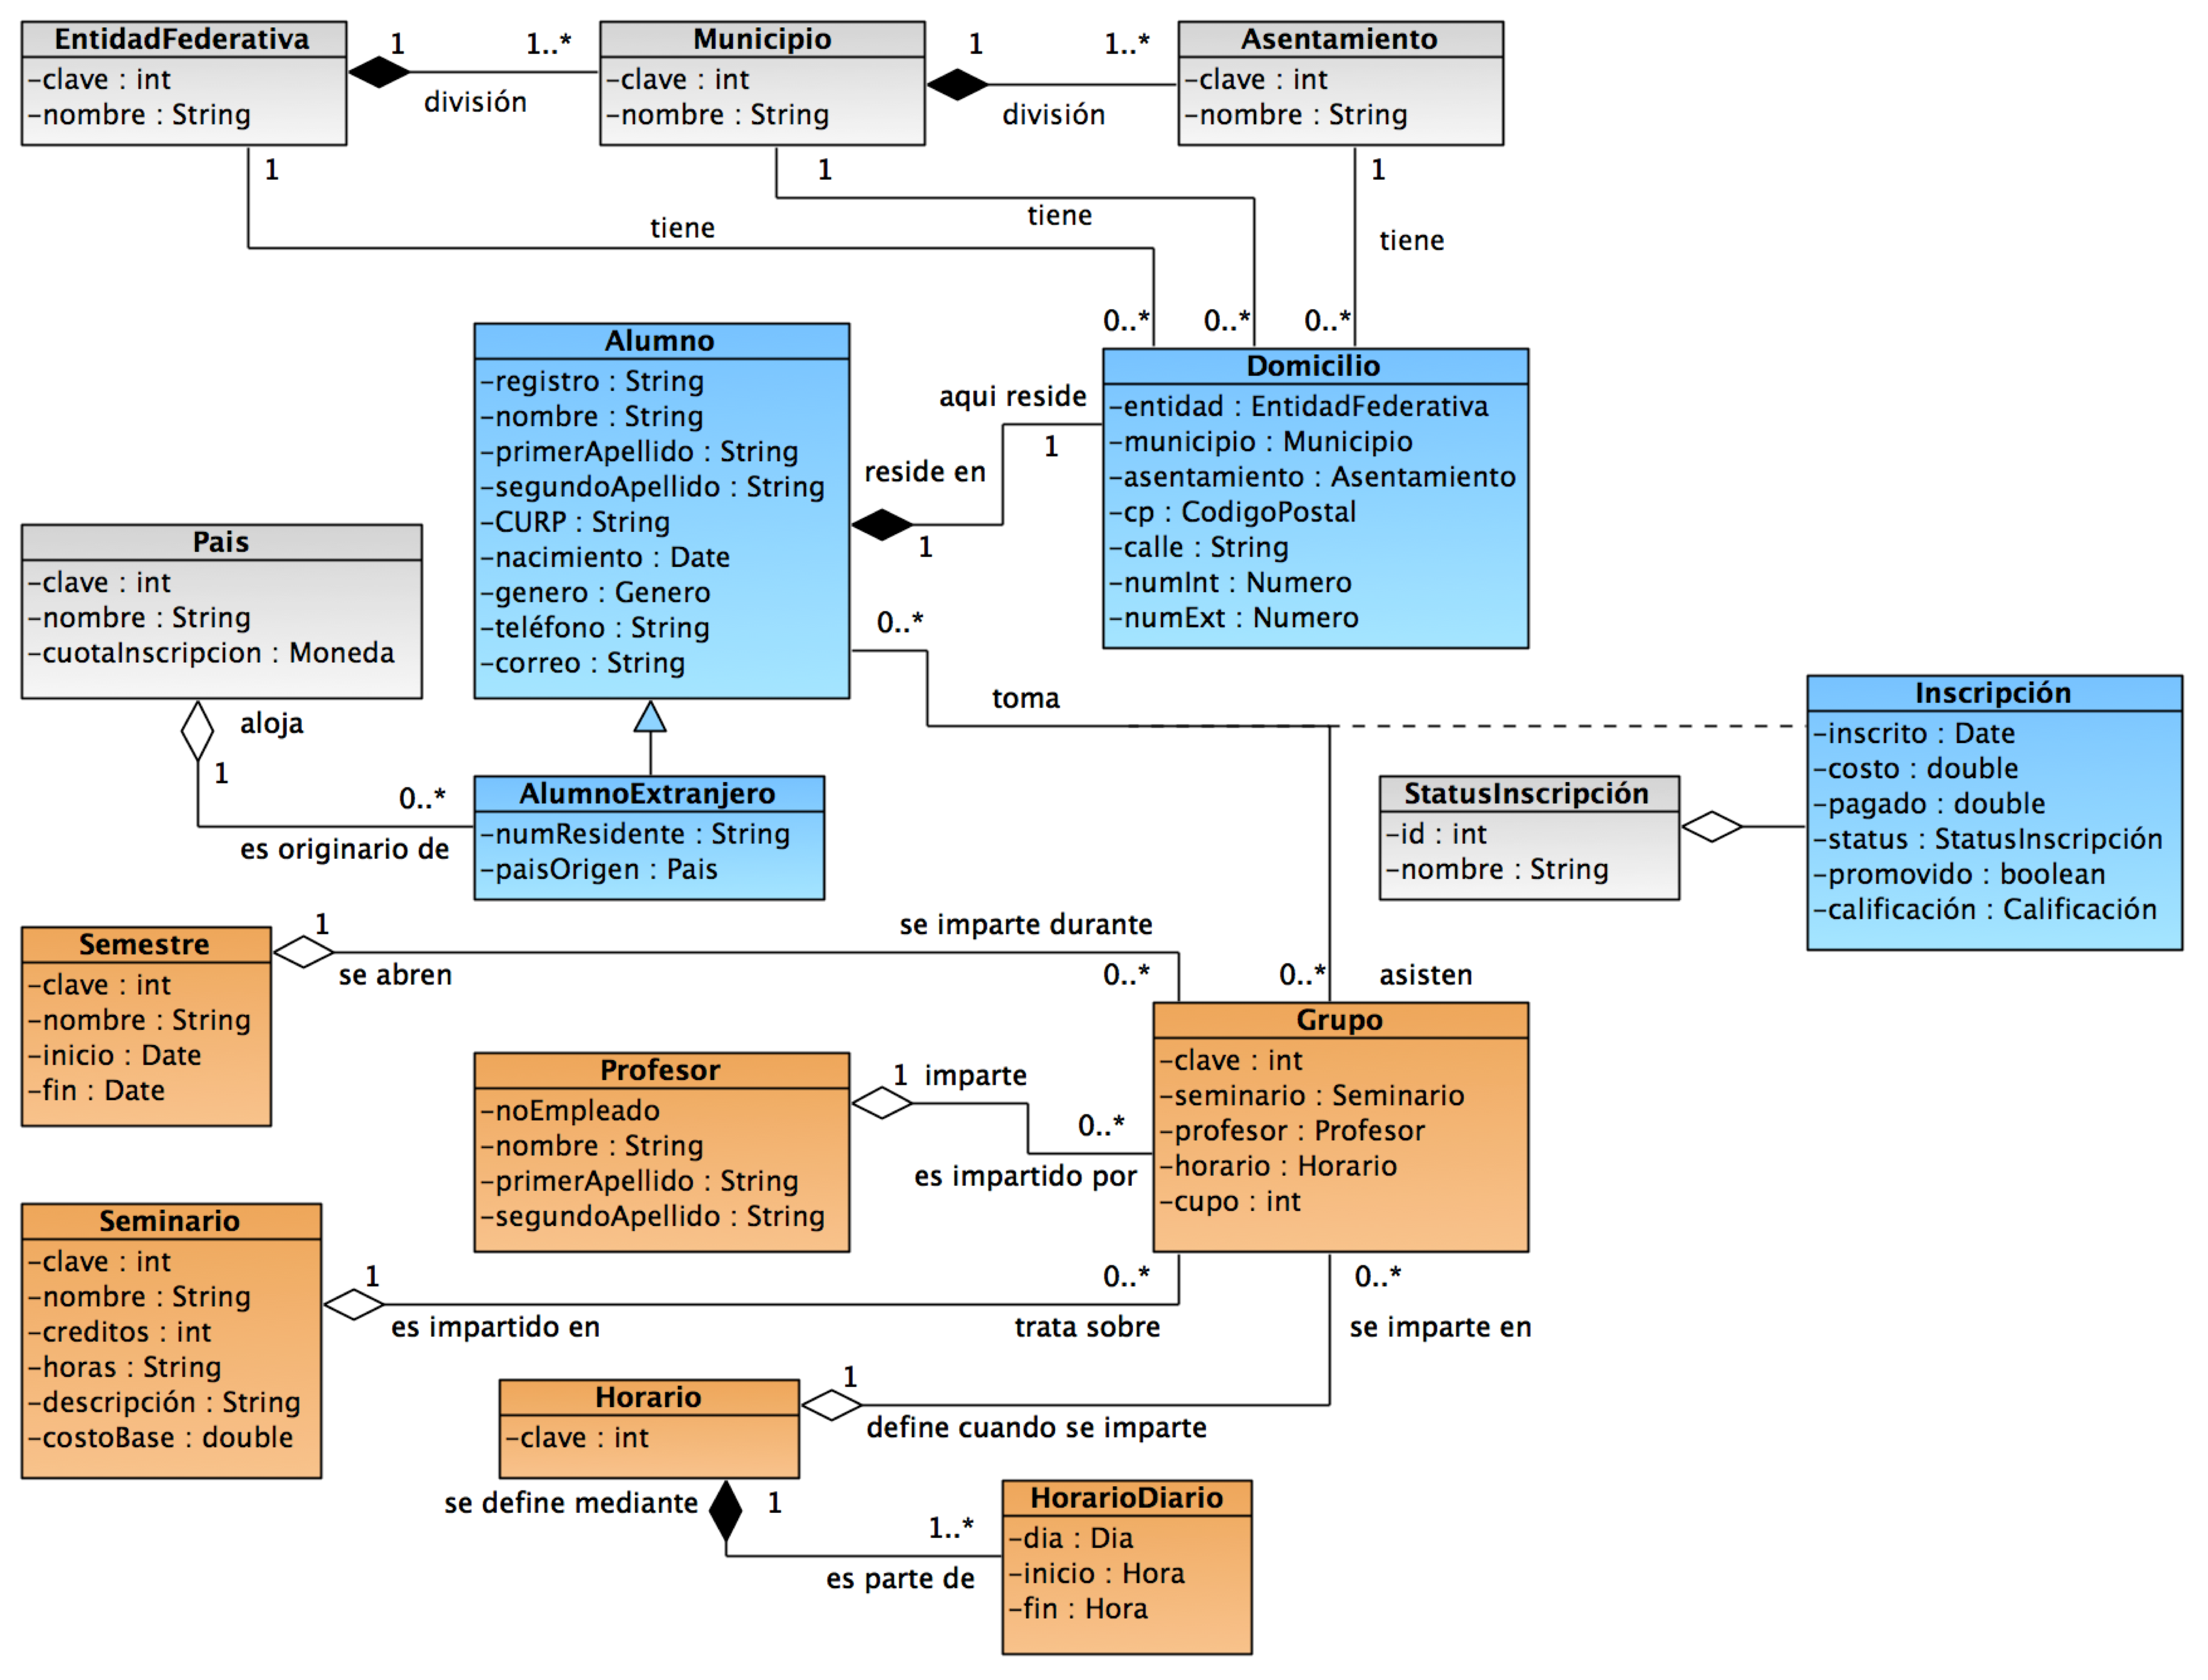
\includegraphics[angle=90,width=.5\textwidth]{images/modeloDelDominioDelProblema}
		\caption{Modelo del dominio del problema}
		\label{fig:modeloDeDominio}
	\end{center}
\end{figure}

\begin{cdtEntidad}{Usuario}{Usuario}
	\brAttr{ID}{Clave Pronim}{Id}{Número de registro utilizado para identificar un usuario}{Sí}
	\brAttr{nombre}{Nombre}{Palabra Corta}
		{Nombre o nombres del usuario.}{Sí}
	\brAttr{primerApellido}{Primer apellido}{Palabra Corta}
		{Primer apellido del usuario.}{Sí}
	\brAttr{segundoApellido}{Segundo apellido}{Palabra Corta}
		{Segundo apellido del usuario.}{No}
	\brAttr{CURP}{CURP}{CURP}
		{CURP del usuario.}{Sí}
	\brAttr{nacimiento}{Nacimiento}{Fecha}
		{Fecha de nacimiento del Usuario.}{Sí}
	\brAttr{Sexo}{Sexo}{Palabra corta}
		{Género del usuario.}{Sí}
	\brAttr{Activo}{Activo}{Booleano}
		{Describe el estao de la cuenta del usuario.}{Sí}
	\brAttr{Fotografia}{Fotografia}{Archivo}
		{Fotografia del usuario para identificarlo.}{Sí}
  \brAttr{Correo}{Correo Electronico}{E-mail}
		{Correo electronico del usuario para la recuperación de contraseña.}{Sí}
  \brAttr{RFC}{RFC}{Palabra corta}
		{RFC del usuario emitido por el SAT.}{Sí}
  \brAttr{Cedula}{Cedula Profesional}{Palabra corta}
		{Cedula que acredita al usuario como un profesionista.}{Sí}
  \brAttr{Contrasenia}{Contraseña}{Palabra corta}
		{Contraseña proporcionada por el usuario para identificarse en el sistema.}{Sí}
	\cdtEntityRelSection
	
	\brRel{\brRelAgregation}{Sexo}{Un \hyperlink{Usuario}{Usuario} tiene un \hyperlink{Sexo}{Sexo}}	
\end{cdtEntidad}
\begin{cdtEntidad}{Sexo}{Sexo}%{}
	\brAttr{Nombre}{Nombre}{Id}{Palabra corta que identifica a un sexo.}{Si}
	\brAttr{Descripcion}{Descripción}{Frase corta}{Descripción que ayuda a comprender que signica cada sexo}{Sí}
	
\end{cdtEntidad}
\begin{cdtEntidad}{CT}{Centro de Trabajo}%{}
	\brAttr{ID}{Identificador}{Id}{Número de registro dado por el sistema al ser registrado.}{Si}
	\brAttr{Calle}{Calle}{Frase corta}{Calle en la que se encuentra el Centro de Trabajo.}{Sí}
    \brAttr{Numero}{Número}{Entero}{Número en la que se encuentra el Centro de Trabajo.}{Sí}
    \brAttr{Colonia}{Colonia}{Frase corta}{Colonia en la que se encuentra el Centro de Trabajo.}{Sí}
    \brAttr{Municipio}{Municipio}{Frase corta}{Municipio en la que se encuentra el Centro de Trabajo.}{Sí}
    \brAttr{Nombre}{Nombre}{Frase corta}{Forma en la que se identifica un centro de trabajo.}{Sí}
    \brAttr{Estado}{Estado}{ID}{Estado en la que se encuentra el Centro de Trabajo.}{Sí}
    \brAttr{Formacion}{Formación}{ID}{Formación que imparte el Centro de Trabajo.}{Sí}
	\cdtEntityRelSection
	\brRel{\brRelAgregation}{Estado}{Un \hyperlink{CT}{Centro de Trabajo} esta en un \hyperlink{Estado}{Estado}}
    \brRel{\brRelAgregation}{Formación}{Un \hyperlink{CT}{Centro de Trabajo} imparte una \hyperlink{Formacion}{Formación}}
\end{cdtEntidad}

\begin{cdtEntidad}{Formacion}{Formación}%{}
	\brAttr{ID}{Identificador}{Id}{Número de la posible formación.}{Si}
	\brAttr{Nombre}{Nombre}{Frase corta}
		{Describe los grados academicos que imparte esa escuela.}{Sí}
	\cdtEntityRelSection
    
\end{cdtEntidad}
\begin{cdtEntidad}{CondicionMigratoria}{Condición  Migratoria}%{}
	\brAttr{ID}{Identificador}{Id}{Número de la posible condición.}{Si}
	\brAttr{Nombre}{Nombre}{Frase corta}{Cadena que nombra una Condición Migratoria.}{Sí}
        \brAttr{Descripcion}{Descripción}{Frase corta}{Cadena que expresa en que consiste  una Condición Migratoria.}{Sí}
	\cdtEntityRelSection
    
\end{cdtEntidad}
\begin{cdtEntidad}{Habilidades}{Habilidades}%{}
	\brAttr{ID}{Identificador}{Id}{Número de la posible habilidad a desarrollar.}{Si}
	\brAttr{Nombre}{Nombre}{Frase corta}{Cadena que nombra una habilidad.}{Sí}
        \brAttr{Descripcion}{Descripción}{Frase corta}{Cadena que expresa en que consiste  una habilidad.}{Sí}
	\cdtEntityRelSection
    
\end{cdtEntidad}
\begin{cdtEntidad}{Idioma}{Idioma}%{}
	\brAttr{ID}{Identificador}{Id}{Número del idioma que entiende.}{Si}
	\brAttr{Nombre}{Nombre}{Frase corta}
		{Es el nombre que se le asigna a un idioma.}{Sí}
	\cdtEntityRelSection
    
\end{cdtEntidad}
\begin{cdtEntidad}{OrigenEtnico}{Origen Étnico}%{}
	\brAttr{ID}{Identificador}{Id}{Número del posible origen étnico.}{Si}
	\brAttr{Nombre}{Nombre}{Frase corta}{Cadena que nombra un origen étnico.}{Sí}
        \brAttr{Descripcion}{Descripción}{Frase corta}{Cadena que expresa en que consiste  un origen étnico.}{Sí}
	\cdtEntityRelSection
    
\end{cdtEntidad}
\begin{cdtEntidad}{Nacionalidad}{Nacionalidad}%{}
	\brAttr{ID}{Identificador}{Id}{Número de la nacionalidad del individuo.}{Si}
	\brAttr{Nombre}{Nombre}{Frase corta}
		{Nombre de la nacionalidad.}{Sí}
	\cdtEntityRelSection
    
\end{cdtEntidad}
\begin{cdtEntidad}{Escolaridad}{Escolaridad}%{}
	\brAttr{ID}{Identificador}{Id}{Número de la escolaridad.}{Si}
	\brAttr{Nombre}{Nombre}{Frase corta}{Cadena que nombra una escolaridad.}{Sí}
        \brAttr{Descripcion}{Descripción}{Frase corta}{Cadena que expresa los grados necesarios para estar en esa escolaridad.}{Sí}
	\cdtEntityRelSection
    
\end{cdtEntidad}
\begin{cdtEntidad}{TipoNota}{Tipo de nota}%{}
	\brAttr{ID}{Identificador}{Id}{Número de la nota.}{Si}
	\brAttr{TipoNota}{Tipo de nota}{Frase corta}{Cadena que nombra el tipo de nota .}{Sí}
        \brAttr{Prioridad}{Prioridad}{Entero}{Numero que establece la prioridad que se le dara a la nota, entre más bajo el numero más alta prioridad tendrá.}{Sí}
	\cdtEntityRelSection
    
\end{cdtEntidad}
\begin{cdtEntidad}{Parentesco}{Parentesco}%{}
	\brAttr{ID}{Identificador}{Id}{Número del parentesco.}{Si}
	\brAttr{Nombre}{Nombre}{Frase corta}{Nombre del parentesco.}{Sí}
	\cdtEntityRelSection
    
\end{cdtEntidad}
\begin{cdtEntidad}{Materiales}{Materiales}%{}
	\brAttr{ID}{Identificador}{Id}{Número del material.}{Si}
	\brAttr{Descripcion}{Descripción}{Frase corta}{Descripción del material.}{Sí}
	\cdtEntityRelSection
    
\end{cdtEntidad}
\begin{cdtEntidad}{Condicion}{Condición}%{}
	\brAttr{ID}{Identificador}{Id}{Número de la condición.}{Si}
	\brAttr{Descripcion}{Descripción}{Frase corta}{Descripción de la condición de un salón.}{Sí}
	\cdtEntityRelSection
    
\end{cdtEntidad}
\begin{cdtEntidad}{Grado}{Grado}%{}
	\brAttr{ID}{Identificador}{Id}{Número del grado.}{Si}
	\brAttr{Nombre}{Nombre del grado}{Frase corta}{Cadena que nombra el grado.}{Sí}
        \brAttr{IDFormacion}{Id de formación}{ID}{Identificador que relaciona el grado con una de las formaciones.}{Sí}
	\cdtEntityRelSection
    \brRel{\brRelAgregation}{Formación}{Un \hyperlink{Grado}{Grado} es parte de una \hyperlink{Formación}{Formación}}
\end{cdtEntidad}

\begin{cdtEntidad}{Estado}{Estado}%{}
	\brAttr{ID}{ID Estado}{Id}{Identificador de cada estado.}{Si}
	\brAttr{Nombre}{Nombre}{Frase corta}
		{Nombre del estado.}{Sí}
    \brAttr{Estado}{Estado}{Booleano}{Verifica si el estado esta registrado en el PRONIM.}{Si}
	\cdtEntityRelSection
		
\end{cdtEntidad}

\begin{cdtEntidad}{CCT}{Clave del Centro de Trabajo}%{}
	\brAttr{CCT}{Clave de Centro de Trabajo}{Id}{Cadena otorgada por la  Secretaría de Educación Pública que identifica un centro de trabajo.}{Si}
	\brAttr{ID_Centro}{ID Centro de trabajo}{ID}
		{Centro de trabajo al que se asocia esta CCT.}{Sí}
  \brAttr{Prestada}{Estado}{Booleano}
		{Describe si esta Clave de Centro de Trabajo la comparten dos o más Centros de Trabajo}{Sí}
	\cdtEntityRelSection
		\brRel{\brRelParticipation}{CCT}{Una \hyperlink{CCT}{Clave de Centro de Trabajo} es de un \hyperlink{CT}{Centro de Trabajo}}
\end{cdtEntidad}
\begin{cdtEntidad}{PrestamoCCT}{Prestamo de Clave del Centro de Trabajo}%{}
        \brAttr{Inicio}{Fecha de inicio del prestamo}{Fecha}{Fecha en la que comienza el prestamo de Centro de Trabjo.}{Si}
        \brAttr{Fin}{Fecha de termino del prestamo}{Fecha}{Fecha en la que termina el prestamo de Centro de Trabjo.}{Si}
	\brAttr{CCT}{Clave de Centro de Trabajo}{Id}{Cadena otorgada por la  Secretaría de Educación Pública que identifica un centro de trabajo.}{Si}
	\brAttr{Receptor}{Receptor}{ID}
		{Centro de trabajo que pide prestada la clave de centro de trabajo.}{Sí}
	\cdtEntityRelSection
		\brRel{\brRelAgregation}{Prestamo}{Una \hyperlink{CCT}{Clave de Centro de Trabajo} es objeto de  un\hyperlink{PrestamoCCT}{Prestamo}}
  \brRel{\brRelAgregation}{Centro de Trabajo}{Un \hyperlink{CT}{Centro de Trabajo} adquier un \hyperlink{PrestamoCCT}{Prestamo}}
\end{cdtEntidad}
%- - - - - - - - - - - - - - - - - - - - - - - - - - - - - 
\begin{cdtEntidad}{AlumnoExtranjero}{Alumno Extranjero}%{}
	\brAttr{numeroResidente}{Numero de residente}{Id}{Número de registro dado por la Secretaría de Relaciones Exteriores a los extranjeros.}{Si}
	\brAttr{paisOrigen}{Pais origen}{\hyperlink{Pais}{País}}
		{País de origen del alumno extranjero.}{Sí}
	\cdtEntityRelSection
	\brRel{\brRelAgregation}{País}{Un \hyperlink{Alumno}{Alumno} es originario de un \hyperlink{Pais}{Pais}}	
	\brRel{\brRelGeneralization}{Alumno}{Un \hyperlink{AlumnoExtranjero}{Alumno Extranjero} es un  \hyperlink{Alumno}{Alumno}}	
	\brRel{\brRelParticipation}{Alumno}{Un \hyperlink{AlumnoExtranjero}{Alumno Extranjero} es un  \hyperlink{Alumno}{Alumno}}	
\end{cdtEntidad}

%---------------------------------------------------------
\section{Modelado de Reglas de negocio}


% !TeX root = proyecto.tex


\cdtInstrucciones{En esta sección describa todas las reglas de negocio identificadas.}


% Tipo: \btDerivation (no aplica Clase), \btEnabler, \btTimer, \btExecutive
% Clase: \bcCondition, \bcIntegrity, \bcAutorization.
% Cumplimiento: \blStrict \blDeferred \blPreAutorized \blPostJustified \blOverride \blGuideline
\begin{BussinesRule}[%
	\brClassification{\btEnabler}{\bcCondition}{\blStrict}
	]{BR-001}{Nombre de la regla de negocio}
	
				% Opciones para nivel: \blControlling, \blInfluencing
	\BRitem[Descripción:] Descripción de la regla. Forma coloquial a manera de reglamento.
	\BRitem[Motivación:] Describa por que es importante la regla.
	\BRitem[Sentencia:] Sentencia formal de la regla.
	\BRitem[Ejemplo positivo:] Indique uno o varios ejemplos en donde la regla se cumple.
        \begin{itemize}
        	\item ...
        \end{itemize}
	
	\BRitem[Ejemplo negativo:] Indique uno o varios ejemplos en dónde la regla no se cumple.
		\begin{itemize}
        	\item ...
        \end{itemize}
	
	\BRitem[Referenciado por:] Liste los casos de uso en donde la regla no se cumple. por ejemplo \hyperlink{CUCE3.2}{CUCE3.2}, \hyperlink{CUCE3.3}{CUCE3.3}.
\end{BussinesRule}




\section{Máquinas de estado}

% !TeX root = proyecto.tex

\cdtInstrucciones{En esta sección describa para cada máquina de estados y a que entidad corresponde. Utilice reglas ECA en el diagrama y elabore el diagrama de estados, una descripción del diagrama, una descripción de cada estado y una descripción de las acciones indicando que casos de uso están involucrados.}

% - - - - - - - - - - - - - - - - - - - - - - - - - - - - 
\subsection{Estados para un préstamo}

En la figura~\ref{fig:edos-prestamo} se muestran ...

\begin{figure}[htbp]
	\begin{center}
		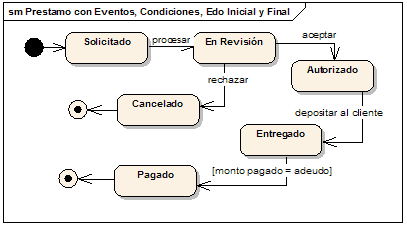
\includegraphics[width=.7\textwidth]{images/edoPrestamo}
		\caption{Máquina de estados de un Préstamo.}
		\label{fig:edos-prestamo}
	\end{center}
\end{figure}

\subsubsection{Estados}

\begin{description}
	\item[Estado:] Descripción del estado.
	\item[...] ...
\end{description}


\subsubsection{Acciones}

\begin{description}
	\item[Acción:] Descripción de la acción indicando el Caso de uso involucrado.
	\item[...] ...
\end{description}




